\documentclass[english]{article}
\usepackage[T1]{fontenc}
\usepackage[latin9]{inputenc}
\usepackage{babel}
\usepackage{graphicx}
\usepackage{float}
\usepackage{multicol}

\graphicspath{{images/}}
\begin{document}
\title{Dissertation Outline}
\maketitle

% Chapter
\section{Motivation and Introduction}

\subsection{History and Literature Review on Semantic Processing in
            Lexical Access}
A review of the literature in regard to these three methodologies:
single word lexical decision, eye-movements, and electrophysiology.

\begin{figure}[H]
\begin{centering}
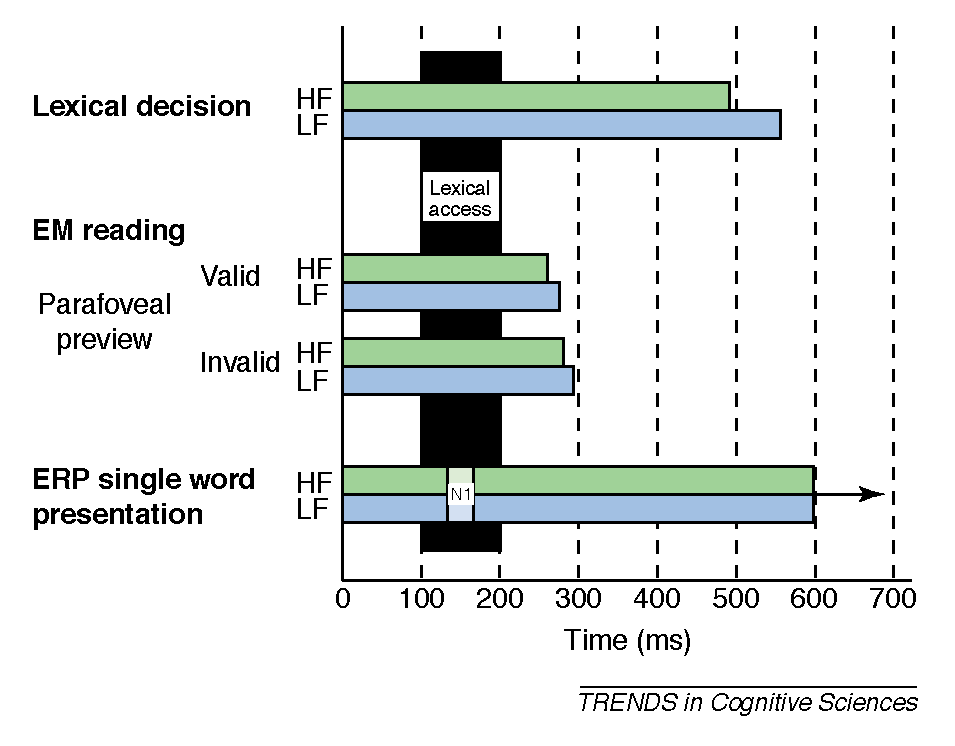
\includegraphics[scale=0.50]{review}
\par\end{centering}
\caption{\label{fig:review} Different Methodology: Different Timecourse}
\end{figure}

\subsection{Methodologies}
Review how each literature tend to interpret their results in terms of a
psychological model of lexical access.

\subsubsection{Single Word Lexical Decision}
\subsubsection{Eye Movements}
\subsubsection{Electrophysiology}

\subsection{Goals}
The goal is to be able to directly compare continous brain activity with a
resultant behavior, which is a composite of the brain response and action.

\begin{figure}[H]
\begin{centering}
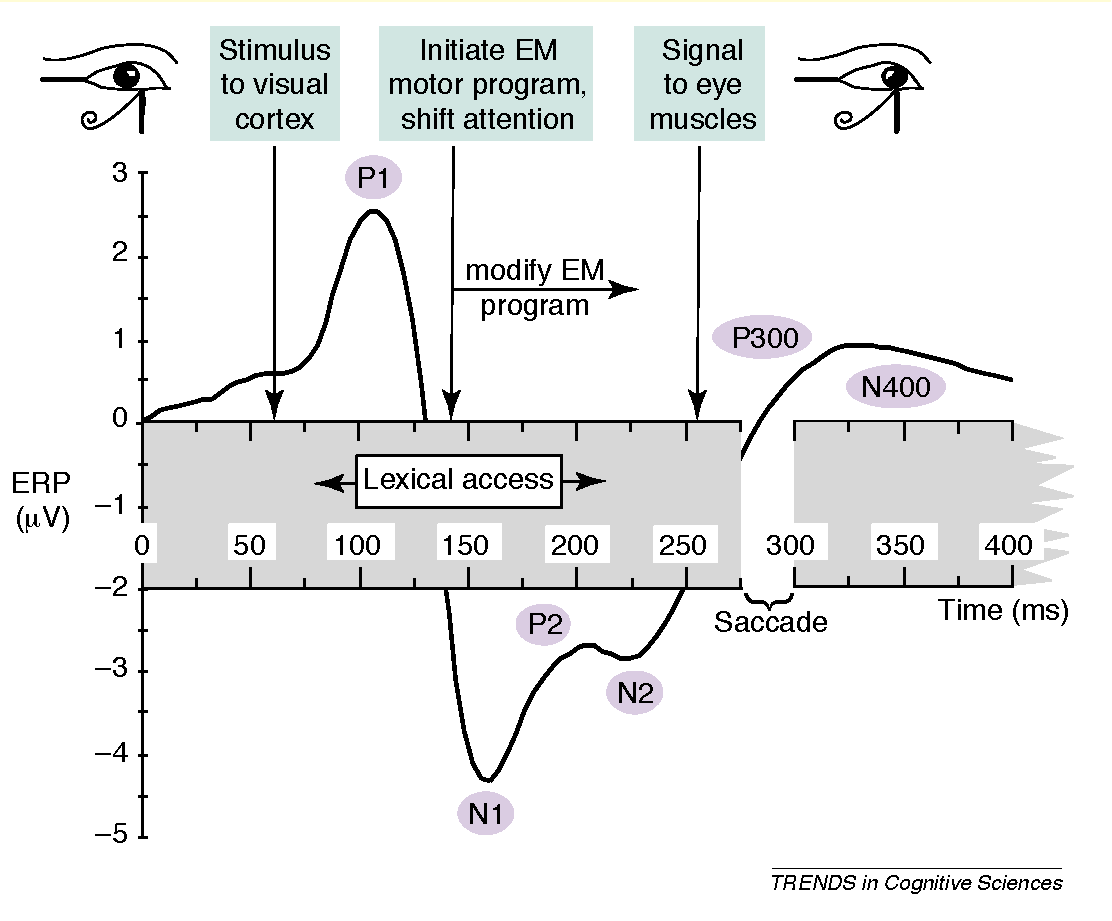
\includegraphics[scale=0.50]{review-goal}
\par\end{centering}
\caption{\label{fig:goal} Goal: Direct Comparison}
\end{figure}

\section{Approaches to Eye-Artifact Removal}
\subsection{PCA}
\subsubsection{What is PCA?}
It is a linear transform of your data such that all components are uncorrelated
with one another. It is a very robust method but it works as a spatial filter
which can be problematic if there are overlapping brain activity in the areas
that are being attentuated.

\subsubsection{Why use PCA?}
Looks for spatial topographies and remove them. This can be used to identify
the eye-artifact from the signal to reduce noise associated with a known cause.

\subsubsection{Review of PCA use in MEG/EEG}
\subsubsection{PCA on Experiment}
This shows the effect of PCA on the waveform of the brain response moving from
fixation cross to hash marks, which later becomes the prime word.
Time region of interest that is used is (-100ms, 30ms).

\begin{figure}[H]
\begin{centering}
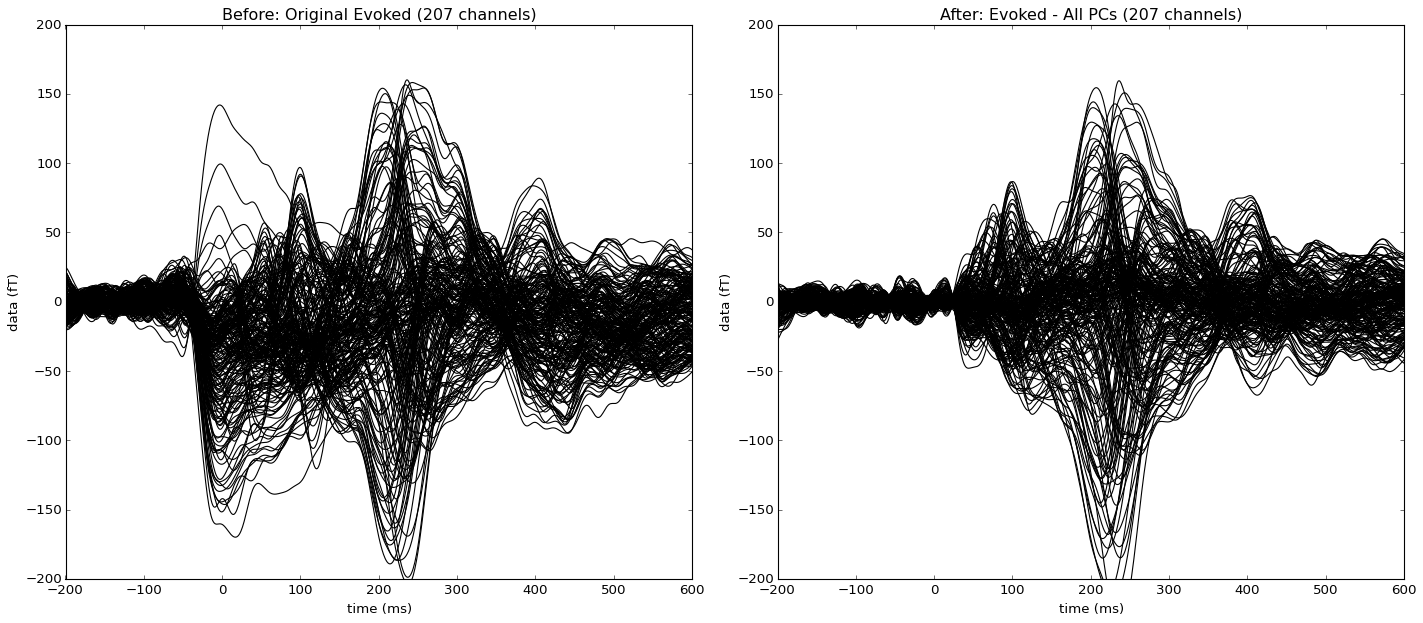
\includegraphics[scale=0.33]{pca-before_after}
\par\end{centering}
\caption{\label{fig:pca-b_a} PCA Before and After}
\end{figure}

These are the topographies of the principal components removed.
\begin{figure}[H]
\begin{centering}
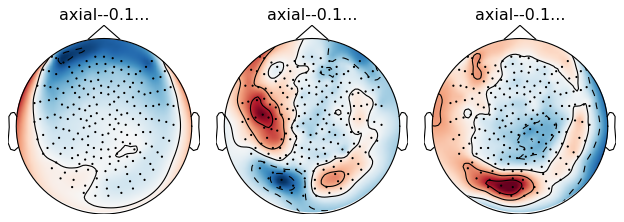
\includegraphics[scale=0.33]{pca-topos}
\par\end{centering}
\caption{\label{fig:pca-topos} PCA Topos}
\end{figure}

This is affected waveform (left) with the PC 0 removed (right).
\begin{figure}[H]
\begin{centering}
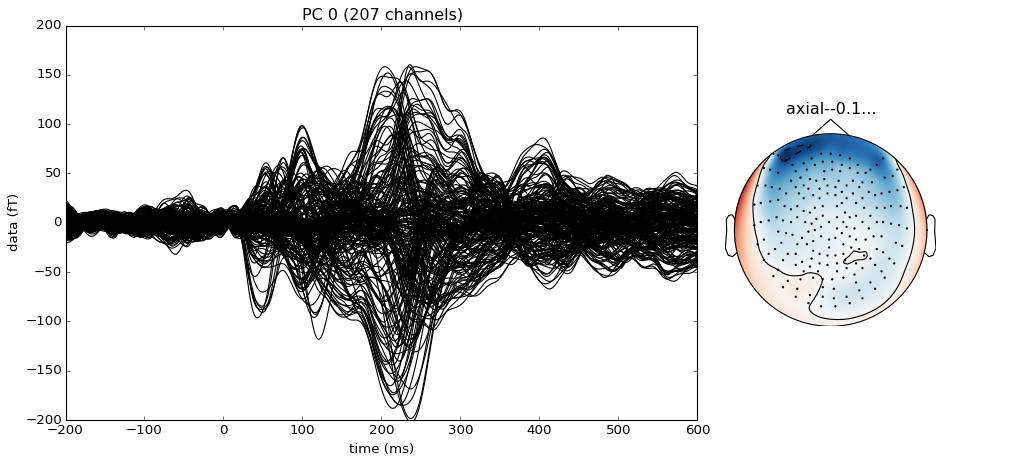
\includegraphics[scale=0.33]{pca-0}
\par\end{centering}
\caption{\label{fig:pca-0} PC 0}
\end{figure}
%
% This is affected waveform (left) with the PC removed (right).
% \begin{figure}[H]
% \begin{centering}
% 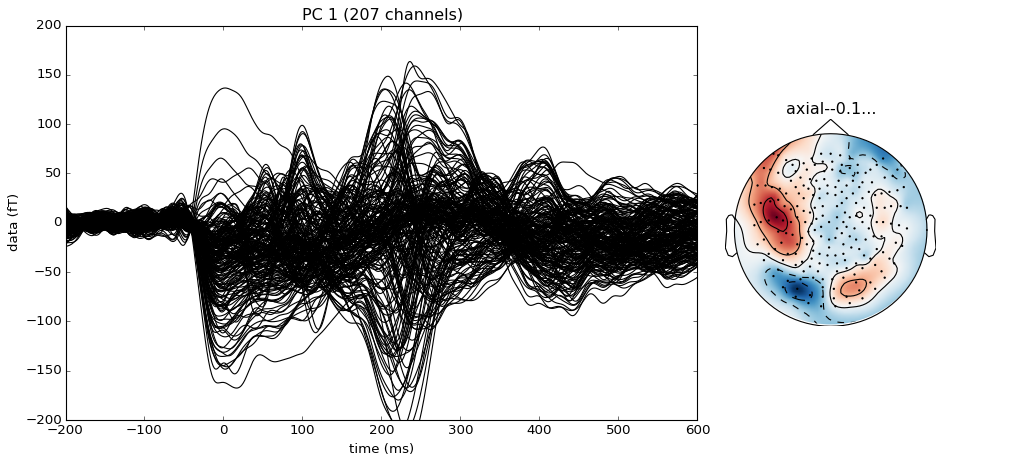
\includegraphics[scale=0.33]{pca-1}
% \par\end{centering}
% \caption{\label{fig:pca-1} PC 1}
% \end{figure}
%
% This is affected waveform (left) with the PC removed (right).
% \begin{figure}[H]
% \begin{centering}
% 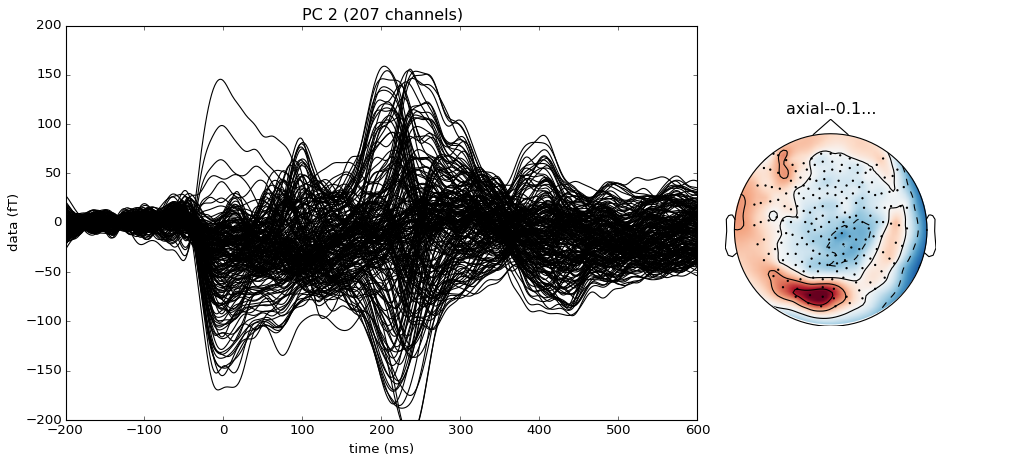
\includegraphics[scale=0.33]{pca-2}
% \par\end{centering}
% \caption{\label{fig:pca-2} PC 2}
% \end{figure}

\subsection{ICA}
\subsubsection{IC Topos}
These are the Independent Component Topographies.
\begin{figure}[H]
\begin{centering}
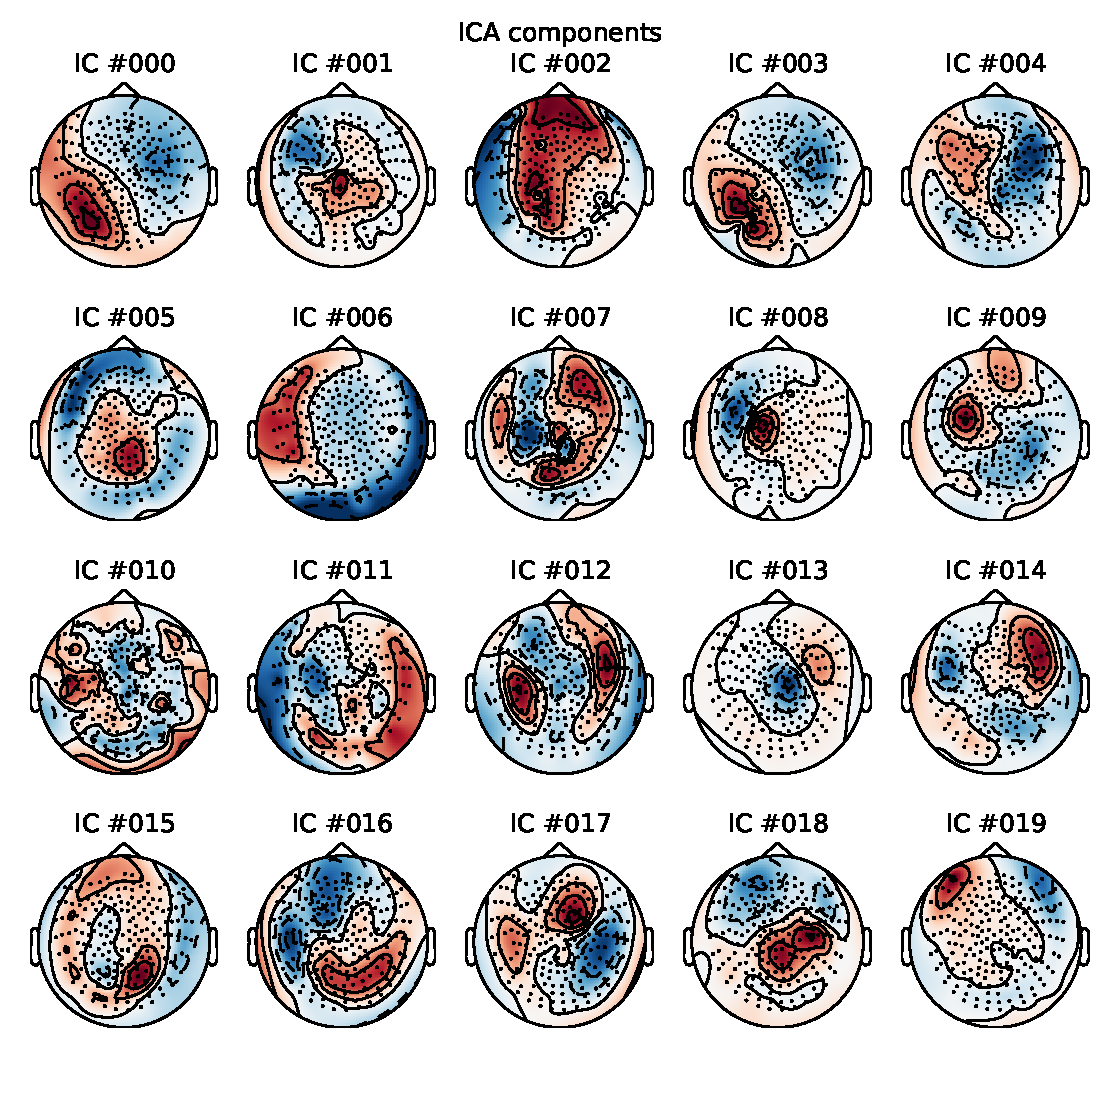
\includegraphics[scale=0.5]{ica-0}
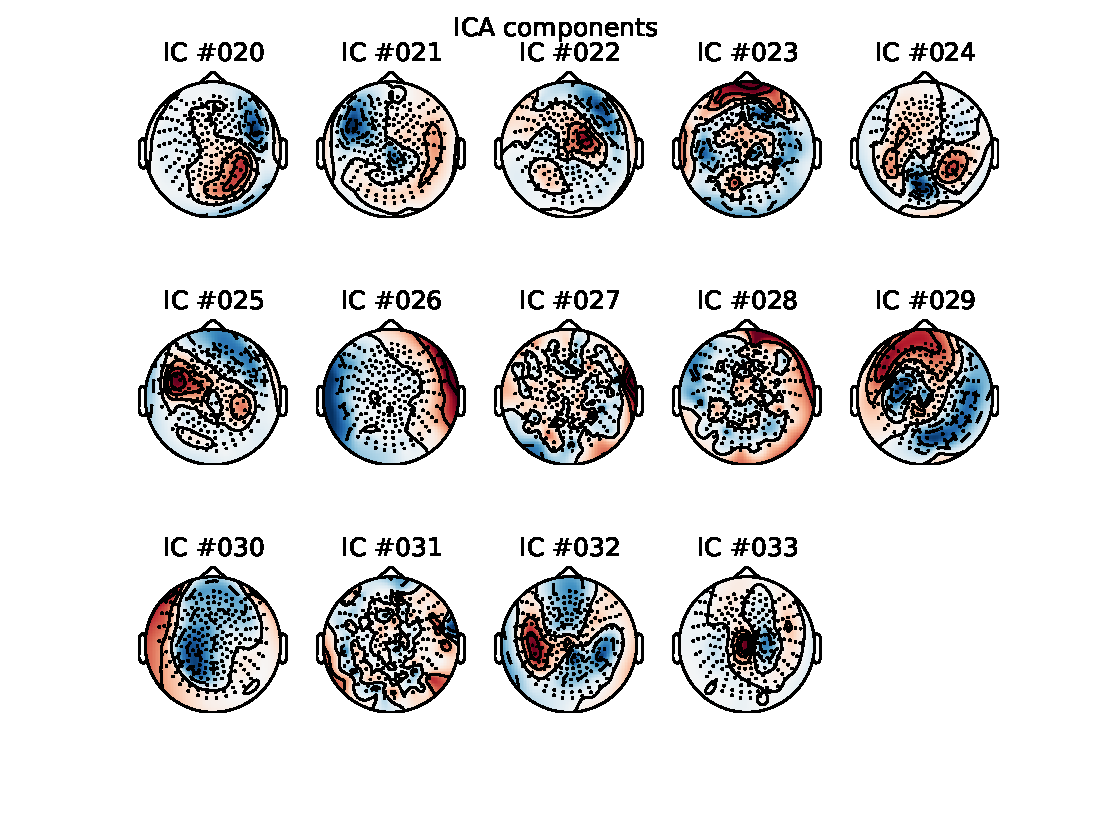
\includegraphics[scale=0.60]{ica-1}
\par\end{centering}
\caption{\label{fig:ica-topo} IC Topos}
\end{figure}

\subsubsection{IC ITC}
These are the Independent Components Inter-Trial Coherence.
\begin{figure}[H]
\begin{centering}
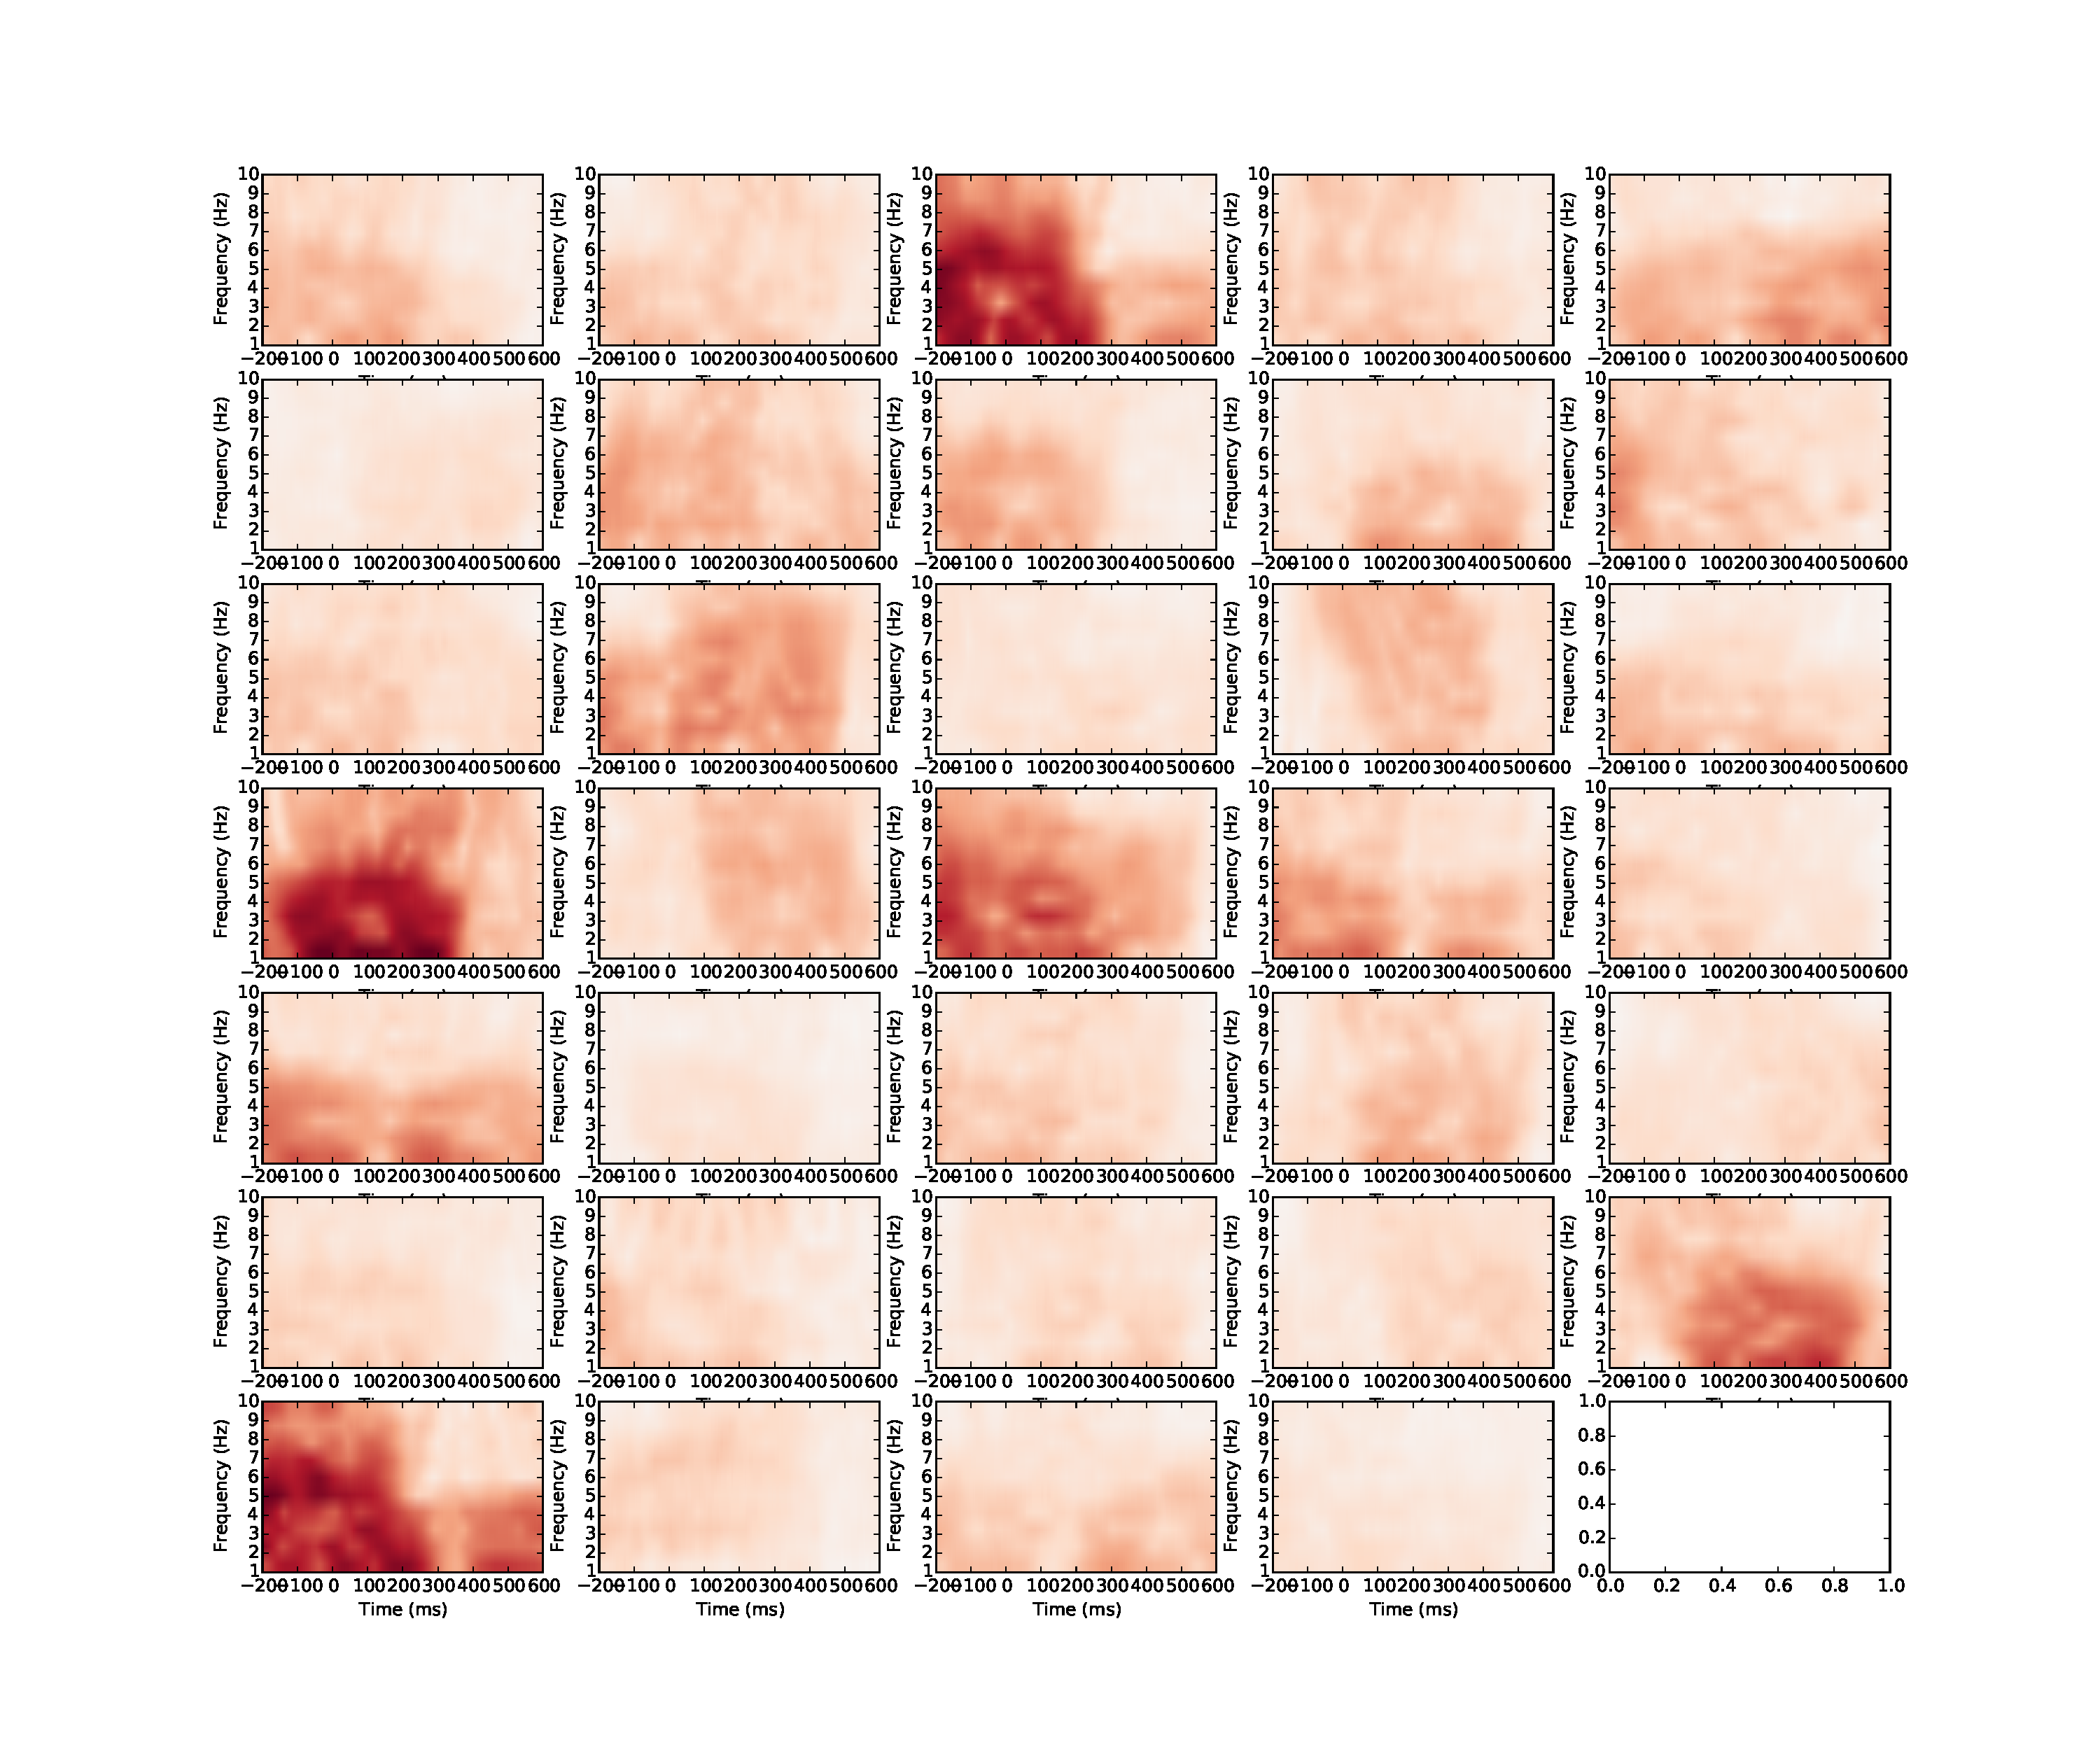
\includegraphics[scale=0.25]{ica-tf}
\par\end{centering}
\caption{\label{fig:ica-itc} ITC}
\end{figure}

% Chapter
\section{Experiment 1: OLDT}

Extend Hoedemaker et al's finding to MEG. This task links the lexical decision
literature to the eye-movement literature but its design.
Our addition is to link these behaviors with some neural correlates.

\begin{figure}[H]
\begin{centering}
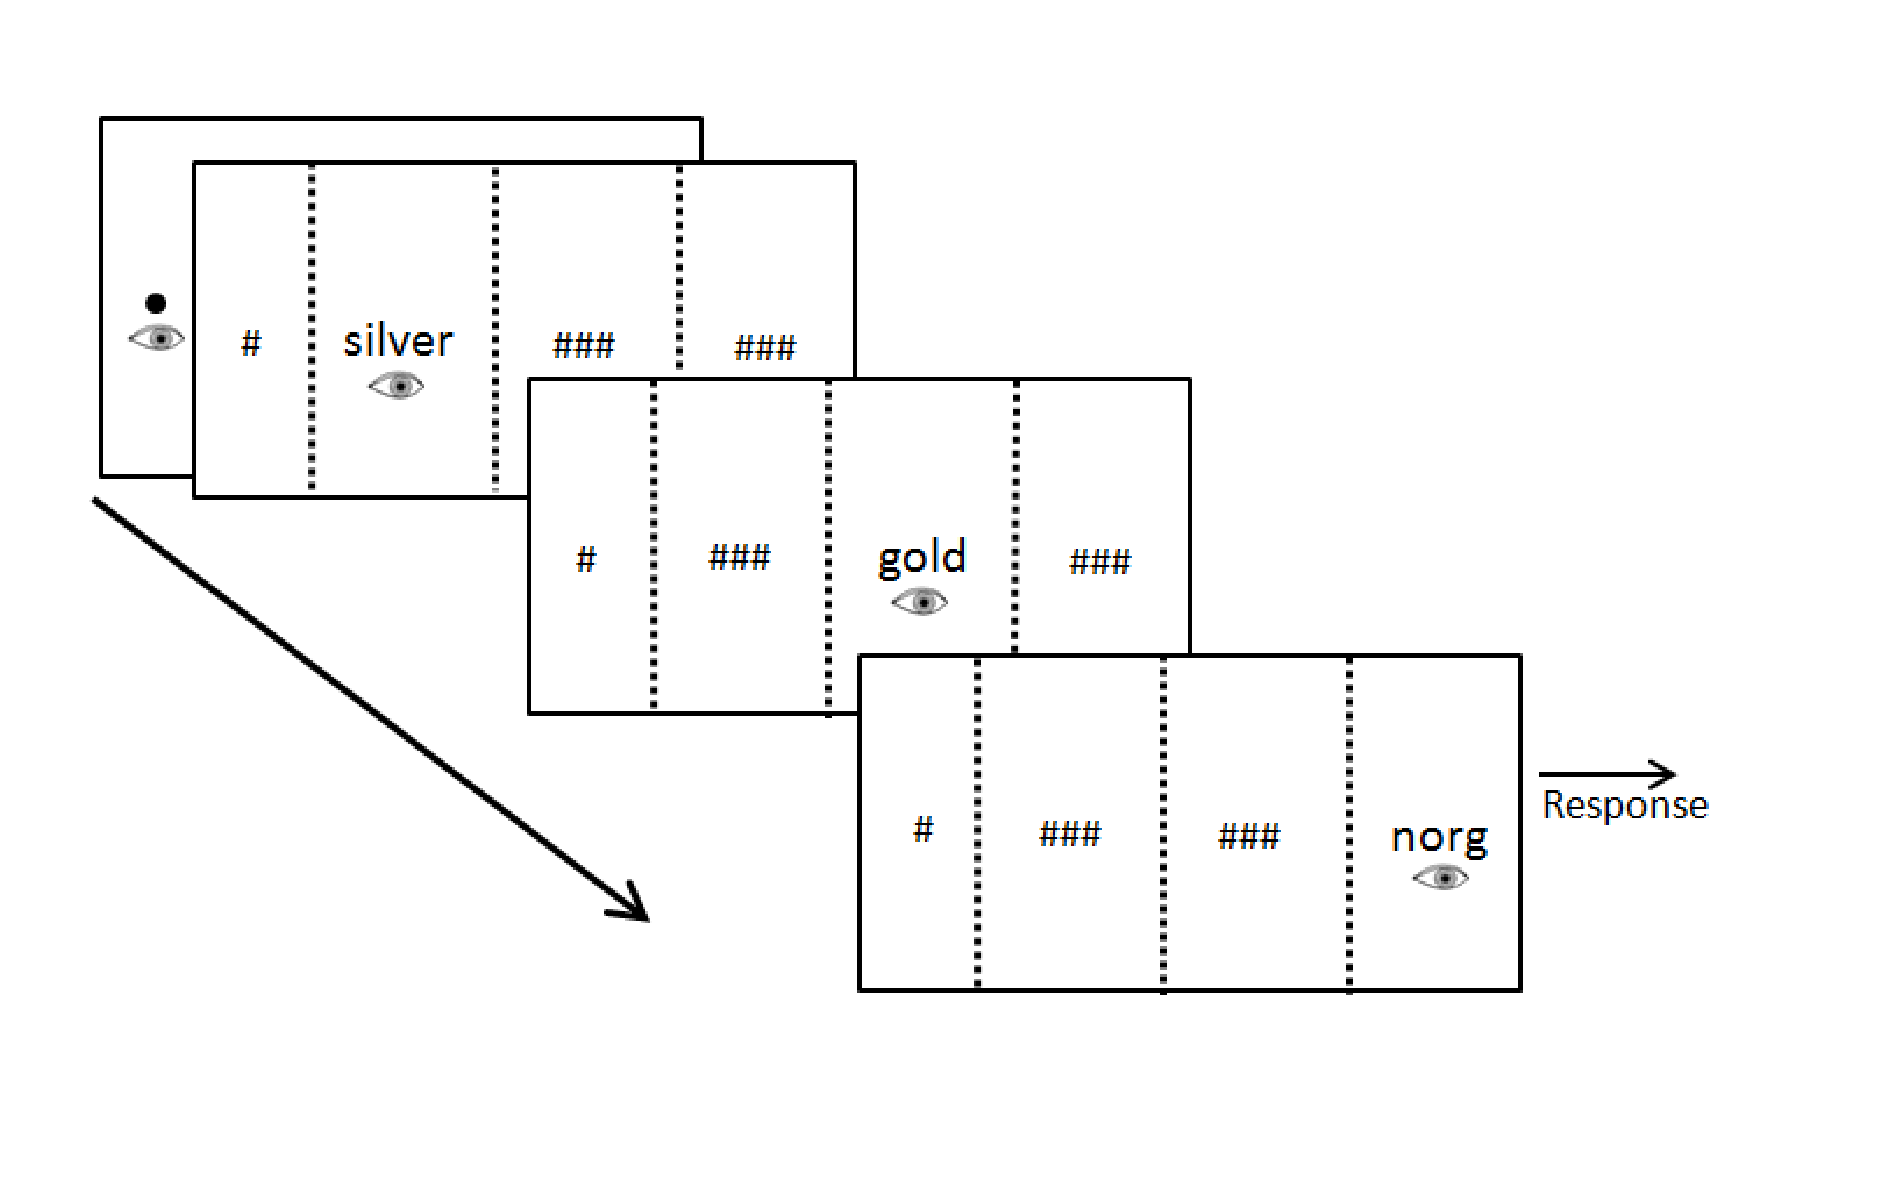
\includegraphics[scale=0.33]{oldt}
\par\end{centering}
\caption{\label{fig:oldt} Ocular Lexical Decision}
\end{figure}

\subsection{Methods}
\subsubsection{Experiment Design}
\subsubsection{Materials}
\subsubsection{Procedure}
\subsection{Analyses}
\subsubsection{Traditional Statistical Approaches}
\subsubsection{Multivariate Approaches}
\begin{figure}[H]
\begin{centering}
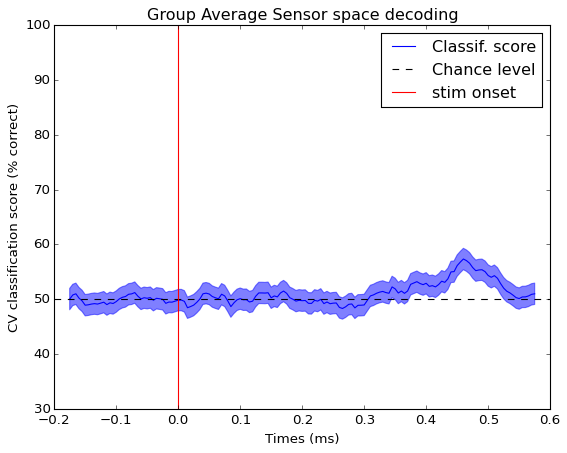
\includegraphics[scale=0.33]{oldt-clf-priming}
\par\end{centering}
\caption{\label{fig:oldt} Group Classification Scores}
\end{figure}

\subsection{Methods}
\subsubsection{Experiment Design}
\subsubsection{Materials}
\subsubsection{Procedure}

\subsubsection{Source-Space}

\subsection{Discussion}

% Chapter
\section{Experiment 2: Simple Sentences}

This takes the OLDT a step further by extending the paradigm to short
declarative sentences. Using semantic association, we can investigate the
effects of semantics on reading time, and the implementation on lexical
access in the brain activity.

\begin{figure}[H]
\begin{centering}
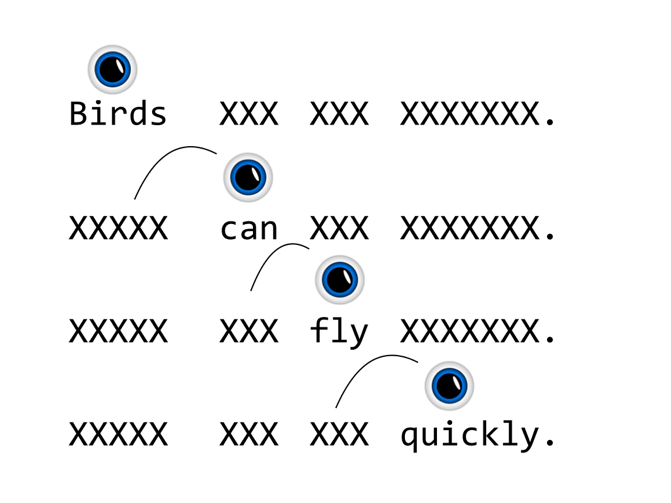
\includegraphics[scale=0.33]{simpsent}
\par\end{centering}
\caption{\label{fig:simpsent} Simple Sentences}
\end{figure}

\subsection{Methods}
\subsubsection{Experiment Design}
\subsubsection{Materials}
\subsubsection{Procedure}

\subsection{Analyses}
\subsubsection{Traditional Statistical Approaches}
\subsubsection{Multivariate Approaches}
\subsubsection{Source-Space}

\subsection{Discussion}

% Chapter
\section{General Discussion, Conclusion, Final Remarks}


\end{document}
